\documentclass{article}

\input{preamble.tex}
\input{Tikz2Code.tex}

\title{Manual \bftt{TikZ2Code.tex}}
\author{MSc. Fausto M. Lagos S.}
\date{\today}

\begin{document}
\maketitle

\begin{abstract}
	\bftt{TikZ2Code.tex} es un conjunto de macros desarrollados para documentar la construcción de figuras con el paquete \bftt{TikZ}, estos macros permiten desarrollar el código de la figura \bftt{TikZ} y agregar de forma automática ésta en un ambiente \bftt{figure} seguido del código o generar un archivo auxilar con el código para insertarlo en el documento en la posición elegida por el autor.
\end{abstract}

\section{A modo de instalación}

Para utilizar los macros \bftt{TikZ2code} no hace falta realizar ningún procedimiento de instalación, basta con incluir \mintinline{latex}{%%----------------------------------------------------------------------
%% TikZ2Code.tex
%% Copyright 2020 Fausto M. Lagos S. - @piratax007
%% piratax007@protonmail.ch
%%
%% Este trabajo puede ser usado, estudiado, modificado y 
%% redistribuido bajo los términos de la Licencia LaTeX Project Public License v1.3c+. 
%% La última versión de esta licencia puede consultarse en
%% http://www.latex-project.org/lppl.txt
%%----------------------------------------------------------------------

\RequirePackage{tikz}
\usetikzlibrary{babel, calc, positioning, fit, arrows, external, shadows}
\RequirePackage{graphicx}
\RequirePackage{tcolorbox}
\tcbuselibrary{listings, minted, breakable, skins}
\RequirePackage{tkz-euclide}
\RequirePackage{tkz-fct}
% puede agregar los paquete tikz que requiera

%%----------------------------------------------------------------------
%% Configuración global del ambiente minted para LaTeX
%%----------------------------------------------------------------------
\setminted[latex]{
style = friendly, 
frame = lines, 
bgcolor = codeback!10, 
linenos = true,
numberblanklines = false,
tabsize = 2, 
fontsize = \small,
resetmargins, 
framesep = 2mm, 
baselinestretch = 1.2,
numbersep = 3pt
}
%%----------------------------------------------------------------------

%%----------------------------------------------------------------------
%% Entradas
%% El subtítulo para la figura
%%----------------------------------------------------------------------
%% Salidas - La figura seguida del código LaTeX que la desarrolla
%%----------------------------------------------------------------------
\newenvironment{tikzPlusCode}[1][]
  {\def\tempCaption{#1}
  \VerbatimEnvironment
   \begin{VerbatimOut}{figure.out}}
  {\end{VerbatimOut}
  \begin{figure}[H]
   	 \centering
     \input{figure.out}
     \caption{\tempCaption}
   \end{figure}  
   \setlength{\parindent}{0pt}
   \begin{minipage}{\textwidth}
     \inputminted{latex}{figure.out}
   \end{minipage}
  }
%%----------------------------------------------------------------------

%%----------------------------------------------------------------------
%% Entradas:
%% Obligatorias - Una cadena ID del código - el nombre del archivo out 
%% que contiene el
%% código LaTeX correspondiente a la figura
%%----------------------------------------------------------------------
%% Salidas: La figura y un archivos ID.out que contiene el código 
%% LaTeX de la figura
%%----------------------------------------------------------------------
\newenvironment{tikzToCode}[1][]
  {\def\tempId{#1}
  \VerbatimEnvironment
    \begin{VerbatimOut}{\tempId.out}}
  {\end{VerbatimOut}
     \input{\tempId.out}
  }
%%----------------------------------------------------------------------

%\tikzexternalize[prefix = figures/] 
%\usetkzobj{all}
% %%----------------------------------------------------------------------
% hace \tkzDrawLine compatible con la librería babel de Tikz
%\makeatletter
%\patchcmd{\tkz@DrawLine}{\begingroup}{\begingroup\makeatletter}{}{}
%\makeatother
% %%----------------------------------------------------------------------

%%------------------------------------------
%% Colores
%%------------------------------------------
\definecolorset{HTML}{}{}{ %
	color1,423E3A;color2,ACB8F1;color3,FF1E12;color4,FF7600;color5,FF8012;myBlue,027FDF; %
	myBlack,181818;myRed,AA3939;myGreen,19B170;myGray,181818;myOrange,FF6302;negative,181818; %
	positive,AA3939;enlace,1D8AEC;url,000000;youtube,C4302B;codeback,A4DCF2;codeframe,0B2C39; %
	structColor,201090;barColor,202122;backColor,8998B5;titlesColor,008100;blueR,1042A6; %
	blueOctave,015794;hlOrange,FFAD7E;citeColor,AA3939 %
}

\definecolorset{rgb}{}{}{ %
	signBlue,0, .25, .53;emeraldGreen,0, .79, .34;topaz,0, .6, .88; %
	indigoDye,.05, .31, .55;indigo2,.13, .53, .41;blueSpider,.15, .27, .43; %
	darkOliveGreen2,.74, .93, .41;ochre,.8, .47, .13;darkOrange,.8, .4, .0; %
	skyblue6,.2, .6, .8;firebrick,.7, .13, .13;blueice,.85, .96, .94; %
	lightcopper,.93, .76, .58
}
%%------------------------------------------} - teniendo el correspondiente archivo en la raíz del proyecto - en el preámbulo para que se disponga de los ambientes \cmdbegin{tikzPlusCode} y \cmdbegin{tikzToCode}

\section{Uso del ambiente \bftt{tikzPlusCode}}

Este ambiente crea una figura seguida del código \textbf{TikZ} requerido para obtenerla.

\begin{exampletwouptinynoframe}
\begin{tikzPlusCode}[Uso de \cmdbs{foreach}]
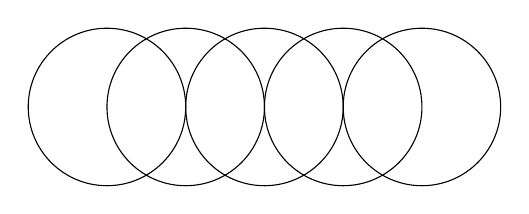
\begin{tikzpicture}
  \foreach \x in {1, 2, ..., 5}{
    \draw (\x, 0) circle[radius = 1cm];
  }
\end{tikzpicture}
\end{tikzPlusCode}
\end{exampletwouptinynoframe}

El ambiente \bftt{tikzPlusCode} recibe como parámetro de entrada obligatorio el subtítulo (caption) de la figura, en su interior se define un ambiente \bftt{tikzpicture} con el código de la figura.

\section{Uso del ambiente \bftt{tikzToCode}}

El ambiente \bftt{tikzToCode} recibe como parámetro de entrada obligatorio un ID para identificar el archivo \bftt{.out} que contendrá el código de la figura \bftt{TikZ}. Este ambiente puede ubicarse o no dentro de un ambiente figure y para presentar el código correpondiente a la figura \bftt{TikZ} debe usarse el comando \mintinline{latex}{\inputminted{latex}{ID.out}} en cualquier parte del documento.

\subsection{Obtención de la gráfica \bftt{TikZ} con el ambiente \bftt{tikzToCode}}

\begin{exampletwouptinynoframe}
\begin{tikzToCode}[idCode]
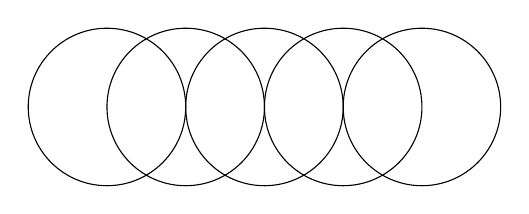
\begin{tikzpicture}
  \foreach \x in {1, 2, ..., 5}{
    \draw (\x, 0) circle[radius = 1cm];
  }
\end{tikzpicture}	
\end{tikzToCode}
\end{exampletwouptinynoframe}

\subsection{Obtención del código generado con el ambiente \bftt{tikzToCode}}

\begin{exampletwouptinynoframe}
\inputminted{latex}{idCode.out}
\end{exampletwouptinynoframe}

\begin{latexPlusCode}
esta es una prueba $x^2$
\end{latexPlusCode}
\end{document}